We instantiated the above described algorithm in the context of logic grid puzzles. 
In that setting there are basically three types of constraints in $\allconstraints$: transitivity constraints, bijectivity constraints and clues, where the first two follow the same structure in every puzzle and the clues are obtained in a mostly automatic way (see Section \ref{sec:holistic}). 
Before defining a cost-function, and the estimation for $g$ used in our implementation, we provide some observation that drove our design decision. 

\textbf{Observation 1: propagations from a single implicit constraint are very easy to understand} Contrary to the clues, the implicit constraints (transitivity/bijectivity) are very limited in form and propagations over them follow well-specified patterns. 
For instance in the case of bijectivity, a typical pattern that occurs is that when $X-1$ out of $X$ possible values for a given function have been derived not to be possible, it is propagated that the last value should be true; this is visualized for instance in Figure \ref{fig:zebrascreen}. 
Hence, in our implementation, we ensure that they are always performed first. Stated differently, $g$ and $f$ are desigend in such a way that $g(C)\geq f(I,C')$ whenever $C'$ consists of only one implicit constraint and $C$ does not. 

\textbf{Observation 2: clues propagate rarely by themselves}
We observed that the automatically obtained logic representation of clues usually has quite weak (unit) propagation strength in isolation. 
This is not a property of the clues, but rather of the final obtained translation. As an example, consider the following sentence: 
``The person who ordered capellini is either Damon or Claudia''. From this, a human reasoner might conclude that Angie did not order capellini. 
However, the obtained logical representation is 
\[\exists p: ordered(p,capellini)\land (p = Damon\lor p = Claudia).\]
This logic sentence only entails that Angie did not order capellini \emph{in conjunction with the bijectivity constraint on $ordered$}.
In the natural language sentence, this bijectivity is implicit by the use of \textbf{the} person which entails that there is only a single person ordering capellini. 

We observed that there is rarely any propagation from sole clues, and that only few implicit constraints are active together with a clue at any time. Hence, when pairing clues to other constraints we always pair it with the set of all implicit (bijectivity, transitivity) constraints.

\textbf{Observation 3: clues are typically used independently from other clues} 
A final observation is that in all the puzzles we encountered, human reasoners never needed to combine two clues in order to derive new information and that when such propagations are possible, they are quite hard to explain, and can be split up into derivations containing only single clues.
The latter is of course not guaranteed, since one can artificially devise disjunctive clues that do not allow propagation by themselves. 
Our algorithms are built to handle this case as well, but it turned out to be not necessary in practice. 
% \tias{smth contrast with 2, e.g. multiple clues WITH impl} 

With these three observations in mind, we devised $f$ and $g$ as follows (where $nc(C)$ denotes the number of clues in $C$): \label{sec:cost}
\begin{align*}&f(I,C) = basecost(C) + |I| + |C|\\
&g(C) = basecost(C) = \left\{\begin{array}{ll}
                               0 & \text{if $|C|=1$ and $nc(C) = 0$}\\
                               20 & \text{if $|C|>1$ and $nc(C)=0$}\\
                               20\cdot nc(C) & \text{otherwise}
                              \end{array}\right.
                              \end{align*}
The number $20$ is taken here to be larger than any reasonable explanation size. 
The effect of this,  is that we can generate our subsets $C'$ in Line \ref{alg:min:for}
 of Algorithm \ref{alg:minexpl} in the following order:
% \tias{'this' refers to f(I,C), 20 is a lot, |I|+|C| < 20} 
\begin{compactitem}
 \item First all $C'$ containing exactly one implicit constraint.
 \item Next, all $C'$ containing exactly all implicit constraints and (optionally) exactly one clue.
 \item Finally, all clue pairs, triples etc. though in practice this is never reached.
\end{compactitem}
Summarized, our instantiation for logic grid puzzles differs from the generic methods developed in the previous section in:
\begin{compactitem}
 \item using a domain-specific optimization function $f$, 
 \item not considering all $C'$ in Line \ref{alg:min:for}, but only considering promising candidates based on our observations,
%  \item 
\end{compactitem}
For the complete non-redundent explanation sequence our tool produces on the running example using these scoring functions, we refer to \url{http://bartbog.github.io/zebra/pasta}. An example of the hardest derivation we encountered (with cost 28) is depicted in Figure \ref{fig:screen2}. It uses several bijectivity constraints for uniqueness of persons, but also for reasoning on the relation between costs and types of pasta, in combination with a clue and three assumptions.
Intuitively, the reasoning happening here can be explained as follows: if Farfalle were to cost \$8, then due to the assumptiosn and bijectivity rotini would cost 16. However, since Damon did not take Farfelle (which we assumed costs \$8), this is in contradiction with the highlighted clue. Hence Farfalle does not cost \$8. 
\bart{remove explanation if space problem BUT MAKE SURE CONCLUSION DOES NOT REFER BACK TO THIS}


\begin{figure}[t]
\centering
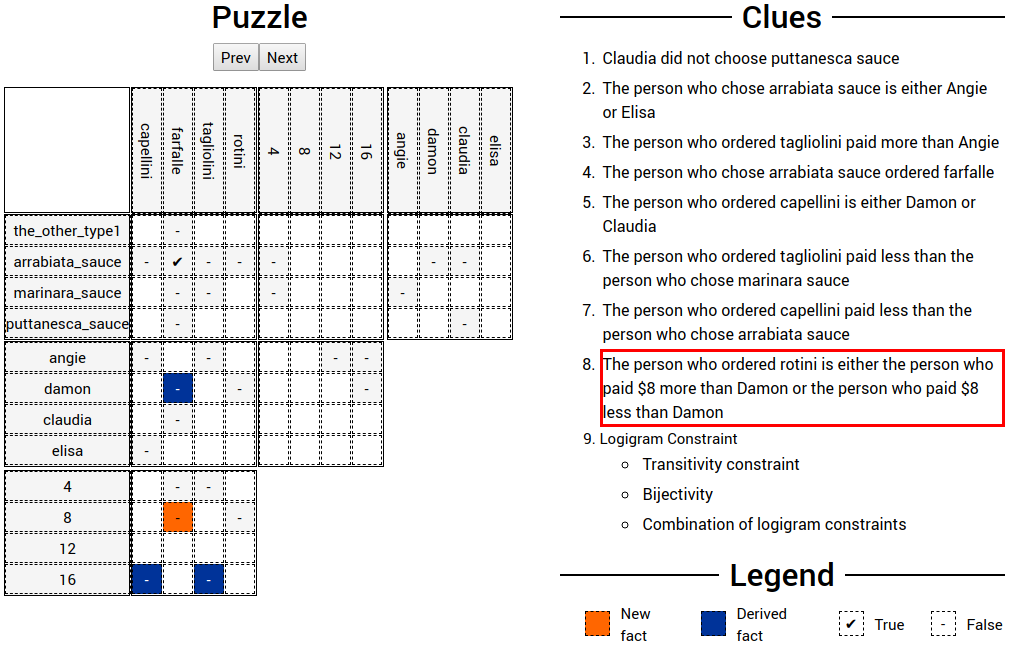
\includegraphics[width=1\linewidth]{zebra_screen_2}
\caption{Demonstration of hard explanation.}
\label{fig:screen2}
\end{figure}


%\tias{We could add a value for the order of the clues, e.g. 0.01*index, to favor higher displayed rules. Also, we could favor 'positive' literals in $N$ by giving these a lower weight, e.g. 0.01 vs 0.1 or smth...}
%\bart{Not so convinced of this... 
%\begin{itemize}
% \item Higher-ranked rules seems quite ad-hoc. Why would they be preferred? This feels more like something we might want to do when we optimize the sequence: ``favour using the same clue twice in a row over switching''. 
% \item  Positive vs negative: no need! This is taken care of automatically!
% The thing is: it not so that positive is ``more natural'' than negative. That really depends on the clue (wehtehr some statement is positive / negative). 
% With the current definitions, you cannot derive the pos from the neg (or the other way round) anymore \textbf{unless} you include the bijectivity csontraint. Hence... using ``the wrong'' of the two costs you $1$. 
%\end{itemize}
%}
%\tias{OK, leave as is}


%\paragraph{Holy Zebra cost function}
%We assume every constraint $c \in C$ has a weight $w(c)$, and we assume every literal has a weight when used as previously derived fact $w_l(f)$, and when it is a newly derived fact $w_r(f)$. The total cost of an explanation is then:
%$$ cost(I', C', A) = w_1*(\sum_{i \in I'} w(i)) + w_2*(\sum_{c \in C'} w(c)) + w_3*(\sum_{a \in A} w(a))$$
%
%The $w_1, w_2, w_3$ can be used to trade-off weights of constraints and facts globally, e.g. to mimic a lexicographic ordering.
%
%In this work, we assume that the weights are manually set based on domain knowledge. For the logic grid puzzles, we prefer small numbers of constraints primarily, so $w_2$ has a high value ($w_2=100$). Among constraints, clues get a weight of $1$ + $0.01$ times their index in the list, such that clues higher in the list get preference. Implicit constraints are even more preferred with a weight of $0.5$ for transitivity constraints and $0.01$ for bijection constraints, as users typically complete the latter immediately.
%Previously used facts are uniformily weighted $w_1=1$ and $w(i)=1, \forall i$. The number of newly derived facts matter less, hence $w_3=0.1$ though with a slight preference for positive literals which get a weight of $w(a)=0.1$ when $a$ is positive, else $w(a)=1$.
%
%Based on this cost function, it is clear that small $C'$ sets should be preferred, but the MUS search does not ensure to find the smallest possible MUS, just that the MUS is minimal. Hence, we will do a 'level-wise' search for increasing constraint set cost $w_2*(\sum_{c \in C'} w(c))$.

%\paragraph{Algorithm modifications}
%\tias{TODO for Bart}





%\paragraph{Old text} 
%Hence, as a measure of difficulty we propose to use a weight function in terms of \textbf{the total number of clues, bijectivity and transitivity constraints, and previously derived facts} needed to derive a new fact. \bart{In fact ,we do not exactly use this measure, since we do not allow combining two clues if there exists some explanation that only uses one}
%The reader should be advised that this is quite a rough approximation; for instance certain clues can be easier than others to reason about (e.g., compare ``Claudia did not choose puttanesca sauce'' with ``The person who ordered rotini is either the person who paid \$8 more than Damon or the person who paid \$8 less than Damon'') or it might be that humans perceive reasoning about clues in general as easier or harder than reasoning about the implicit (bijectivity and transitivity) constraints presents in logic grid puzzles. While researching better measures is an interesting topic, it falls out of the scope of the current paper. Moreover, many ideas of the current work remain valid when the actual measure is changed. 
%Our observatoin from below, that using second-order logic tools such as e.g. \cite{proB,kr/BogaertsTS16} to find cost-optimal justifications is an option remains valid as long as the cost-functoin is expressible in (a sufficient extension of SO). Yet, due the high complexity, is not a direction we explored. 
%\bart{Actually, I would really like to try this sometimes. The complexity argument is valid. But since we have small domains it is actually not so relevant... Maybe it works well. In that case it would yield good explanations!  }
%\tias{OK, where?}

% 
% \paragraph{Simple sequence vs simple steps}
% In the above, we focused on generating and defining understandability of a single step in the reasoning process. 
% However, in its most general form, we would like to optimize the understandability of the entire sequence of explanations. 
% For this, even defining a measure seems to be a very hard task (for instance, is the understandability of a sequence related to its most difficult step or to its average difficulty? Sometimes even the ordering of the steps might make a difference for humans, even though the actual steps are the same, ...). 
% Furthermore, even if we fix a measure, the problem of holistically optimizing a sequence of explanation steps is much harder than optimizing a single step since there are exponentially more sequences. 
% Therefore, in the current paper, we take a greedy approach where at each step, the best next possible explanation is chosen, without taking global optimality of the sequence in mind. The results we obtain this way are satisfying. 
% \bart{And already say something about postprocessing?}
% 
